\documentclass[12pt]{article}
\title{Report iteration 3 - SWOP}
\author{Dieter Geboers, Wouter Schaekers, Stefaan Truijen\\ - \\ Professor: Tom Holvoet \\ Project Advisor: Marko van Dooren}
\date{2012-04-06}
\usepackage[pdftex]{graphicx} % fotootjes
\usepackage{fancyhdr} % coole template
\usepackage[top=20mm,bottom=20mm,left=20mm,right=20mm]{geometry} % size and margins
\usepackage{hyperref} % for urls
\usepackage{listings} % code style
\pagestyle{fancy} % ook coole template
\begin{document}
\maketitle

\section{Preface}
This iteration is the final one. The new assignment instructed us to update our project so that it is able to support multiple campuses on hospitals. With this new feature came a new feature for doctors as well. Doctors gained the ability to travel between campuses. They also get a say in their behaviour concerning travelling between campuses: go back and forth between all campuses, or rather have an own schedule concerning locations? \\
\newline Preemptive scheduling and tasks that support multiple priority levels were not part of our assignment as we're a team of three members. \\
\newline We delivered a report on the refactoring changes we planned to execute during this iteration as well as two test scenarios for our system. However, as we changed the way the system works, the test scenarios were forced to be adapted. We also thought that it would be best to create an additional testing scenario to prove that the "basics" are not the only thing we can do. \\
\newline Our project advisor, Willem Penninckx, was replaced by Marko van Dooren for this iteration due to illness. We had some very constructive meetings with them both and are very thankful for the insight they gave us. Especially when we started to deviate from the core of the  project by over thinking some of the design decisions.\\
\newline For the first time in our SWOP history we can say with confidence that everything works like it should and there are no missing features.

\pagebreak
\tableofcontents
\pagebreak

\section{Introduction}
During the feedback session of iteration two, some major (asw ell as minor) issues with our code and design floated to the surface:
\begin{itemize}
\item{MachinePool had hard coded methods to create different types machines;}
\item{There were no system sequence diagrams available;}
\item{The UML of the domain layer did not have any relevant methods on it;}
\item{The implementation of Warehouse was lacking in a lot of aspects: }
\begin{itemize}
\item{When an activity that required something from a warehouse got scheduled, there were no items removed from that warehouse;}
\item{The way Warehouse kept track of it's items and their maximum capacity was hardcoded;}
\item{The system for creating stock orders and delivering them to the warehouse wasn't implemented successfully;}
\item{\dots}
\end{itemize}
\item{The unit for time (milliseconds) used in the system was nowhere documented.}
\item{Some methods and controllers required the same set of parameters and instead of an object that groups them together, they were all mentioned explicitly;}
\item{...}
\end{itemize}
We have taken all of the above (and more) into account while implementing iteration three to make certain that our hard work would not have been in vain.
In this report we'll motivate the necessity of changes we have put the project through. Also, we'll try to give some other solutions for the problems we encountered that caused us to create the system as it is. We'll then draw a conclusion and leave it at that. \\
\newline As for the amount of time we spent working on this iteration in detail, we refer to \url{http://code.google.com/p/swop-dswx/wiki/WorkingHours} . For a high level view, here's a table:
\begin{center}
    \begin{tabular}{ | l | l | l | p{100mm} |}
    \hline
    Dieter & Stefaan & Wouter\\ \hline
    85h & 110h & 110h\\
    \hline
    \end{tabular}
\end{center}
There has been a total of 150 hours.

\section{Package visible constructors}
We decided to make as many constructors as we could package visible only. Doing this denies the creation of the affected objects by any unwanted classes/people efficiently. However, the lack of friend classes and friend packages in Java made it impossible to protect every constructor of every class in such a way. \\
If such a class or method exists, there will be documentation stating that the method or class in question should never be used outside of the domain layer.\\
For example: once Machine objects get created, they are added to a MachinePool immediately. The responsibility of assigning every Machine to a MachinePool lays with the MachinePool itself.

\section{Creational design patterns}
The following problem presented itself to us a couple of times while developing a plausible design for the assignment: what is a \emph{clean} way to allow users to create new objects of certain dynamically changing classes? For example: how can we make sure that the user  has the ability to create a new ultra sound scanner without making the domain inconsistent or giving too much responsibility to the user interface?\\
An answer to this question is implementing a creational design pattern. We decided to use a builder pattern for the creation of new Machines and an abstract factory pattern for the creation of new Users, Treatments, MedicalTests.\\
The builder mentioned above is nothing like the StandardHospitalBuilder, ExtendedHospitalBuilder, WarehouseBuilder, UserManagerBuilder,... that you may have noticed in the source code of our project. In fact, they're nothing alike. The latter builders are templates for an initialised system to avoid a bunch of code duplication across different testing units.\\
\newline Without further a due, we will now briefly discuss the creational patterns mentioned in the paragraph above.

\subsection{User factories and user manager}

\begin{figure}[h!]
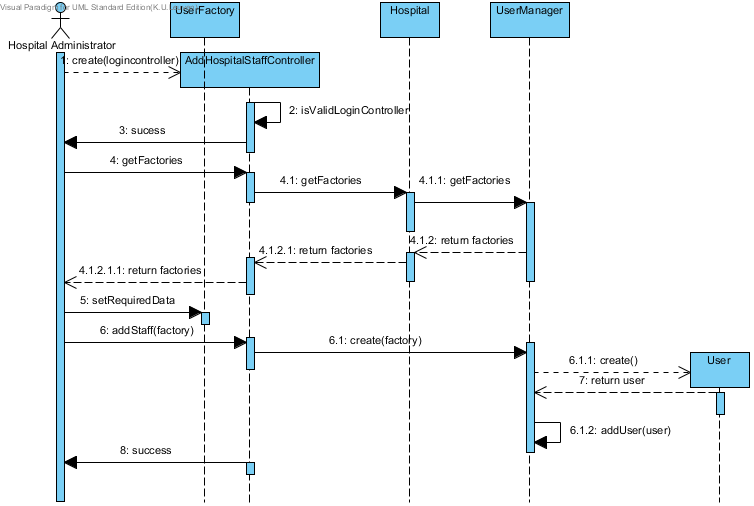
\includegraphics[width=175mm]{addstaff.png}
\caption{The sequence diagram from the add hospital use case demonstrates how user factories are to be used and how they work in the domain layer.}
\label{addHospitalStaffSD}
\end{figure}

First, let's take a look at the sequence diagram of add new hospital staff above. We can see that the hospital administrator asks a list of all available factories, then selects the kind of factory he would like to create a new staff member from, next sets the required parameters and then lets the system create such a user.\\
The creation of the actual User object is the responsibility of the UserManager. This makes it easy to make certain that, when the user uses the public controller API, it's impossible to create a new User object that's not kept in a UserManager.

\subsection{Machine builder and machine pool}
Blood analysers, x-ray scanners and ultra sound scanners all have the same signature in their constructors. They also do not have any specific characteristics other than their types. This is the reason we chose to use a builder design pattern as a solution to the creational problem described in the beginning of this chapter.\\
It is also important to note that the constructor and build()-method of each builder is package visible only. This means no new MachineBuilder objects can be created without going through the MachinePool. Also the constructors of each of the machine types are package visible only. The combination of these visibility limitations means that, analogous to the case with UserFactory and UserManager, creating a new Machine or MachineBuilder object without registering it in a MachinePool is impossible.\\
Alas, the visibility in Java is not what it could be. We were forced to make the Machine classes themselves public as we require Machine objects in other packages. In particular, packages that contain TaskDescriptions come to mind, but more on that later.

\begin{figure}[h!]
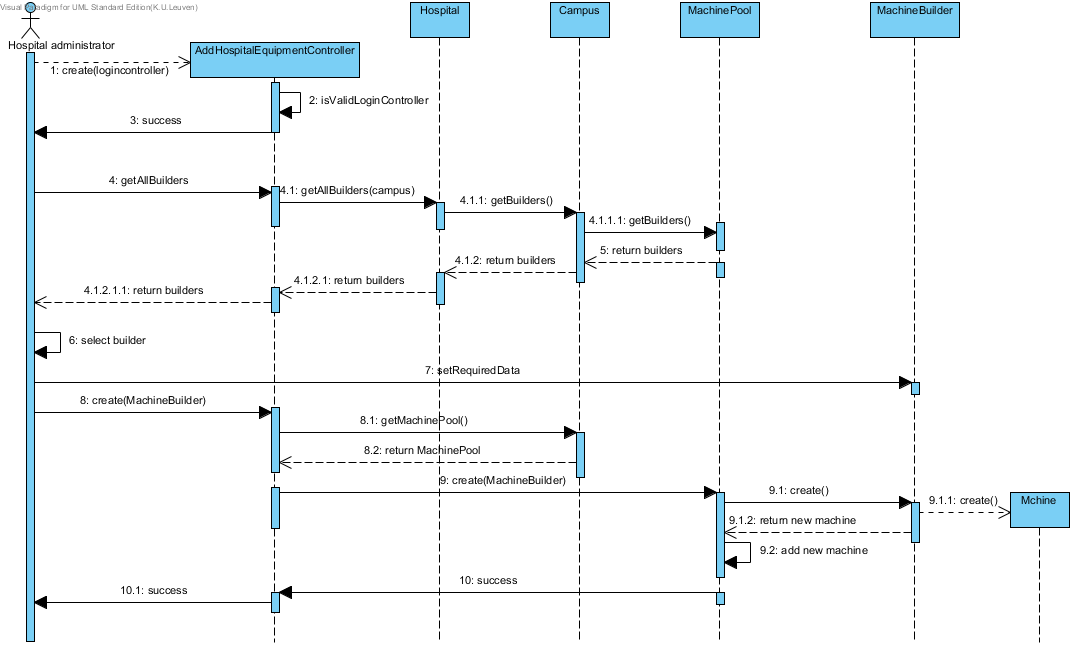
\includegraphics[width=170mm]{addequip.png}
\caption{A sequence diagram of the add equipment use case}
\label{addequipment}
\end{figure}

\subsection{Medical test factories and patient files}
When a doctor wants to order a new medical test for a patient, he or she will create a new OrderMedicalTestController. This controller allows the doctor in question to get all existing medical test factories. These factories are stored in the Hospital class and should be added manually at initialisation time before any use cases can be executed.\\
Once said factories have been acquired from the controller, the doctor can specify the required details in order for the medical test he's about to order to be exactly as he or she would like it to be. The doctor then calls upon the controller one more time, giving it the pre-set MedicalTestFactory. The controller passes this factory on to the task manager. The task manager executes the create()-method. This method generates a new MedicalTestDescription. This description is then stored in a new Task. The Task is then initialised (which means it will be stored in the patient file of the patient who the medical test is for).\\
We would have preferred for the create()-method to have limited visibility. Once again Java does not provide us with the possibilities to do so. Therefore we have equipped it with the \texttt{@Deprecated}-annotation so that, should someone try to call this method, they will see that it's not meant to be called. The documentation of the create()-method also informs the reader of this.\\
Like before, this way of things allows for a reliable domain layer to be constructed and maintained throughout the execution of the program. No MedicalTest objects will ever exist without there being a Task, as well as a PatientFile, to store them. The way Tasks are created (by first creating descriptions and then transforming them into Tasks in the TaskManager) also assures that Tasks never exist created without a TaskManager keeping track of them. Also, we would like to note that the constructor of Task is package visible within the scheduler.tasks package to aid in achieving this goal.
\subsection{Treatment factories and diagnosis}
Treatment factories allow doctors to create treatments that are always linked to diagnose similar to the way medical test factories allow doctors to create medical tests that are always linked to a patient file.\\
The doctor creates the appropriate controllers and asks them for the treatment factories available in this hospital. Just like is the case with medical test factories, these treatment factories are to be initialised at system initialisation time before any use cases can be ran.\\
The doctor chooses one of the given treatment factories and sets the required data. Then the doctor gives the factory back to the PrescribeTreatmentController, who then in turn, gives it to TaskManager. The TaskManager then creates a description from the factory and transforms it to a Task. The created Task gets initialised, which causes it to be linked to the diagnose it was created for.
\subsection{Diagnosis and patient files}
No Diagnose objects should exist without there being a PatientFile object to store them. The sequence diagram below demonstrates how assuring this consistency happens when the controllers are used properly:

\begin{figure}[h!]
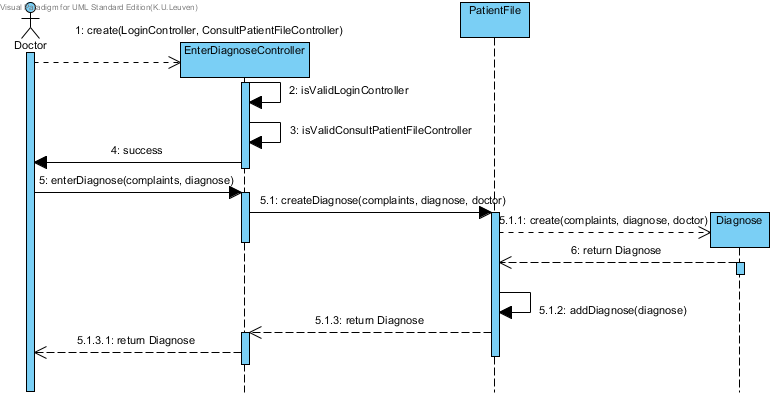
\includegraphics[width=170mm]{enterdiagnose.png}
\caption{The sequence diagram of the enter diagnose use case demonstrates how no diagnose can be created without a patient file storing it.}
\label{enterdiagnose}
\end{figure}
\subsection{Warehouse builder and campus}
Warehouses should not exist without a StockProvider (see later). Also a campus should always have a warehouse. To make this possible we use WarehouseBuilder objects at initialisation time. These warehouse builders are not design pattern builders but merely a way to assure the desired consistency mentioned above at creation time.

\section{Task}
Task object represent task concepts from the real world. Tasks are created from descriptions and are stored in the TaskManager. Tasks can undergo 2 transformations in their lifetimes. When they are created, they are regarded to as queued tasks. When the opportunity presents itself, the queued task becomes a scheduled task. Once the scheduled task has been executed, it becomes a finished task.
\subsection{Generic tasks versus a hierarchy of tasks}
Tasks come in many different forms. In the last iteration, we worked with a hierarchy of Task objects. For example: UnscheduledMedicalTestTask, ScheduledMedicalTestTask, UnscheduledTreatmentTask, ScheduledTreatmentTask, \dots . During a meeting with our project advisor, we came to the conclusion that such a hierarchy is not very desirable and violates the GRASP patterns. We then chose to work with a generic Task class: \texttt{Task<? extends TaskDescription>}. "Tasks from task descriptions".\\
The class diagram from Tasks and their descriptions can be found in figure ~\ref{taskuml} .

\begin{figure}[h!]
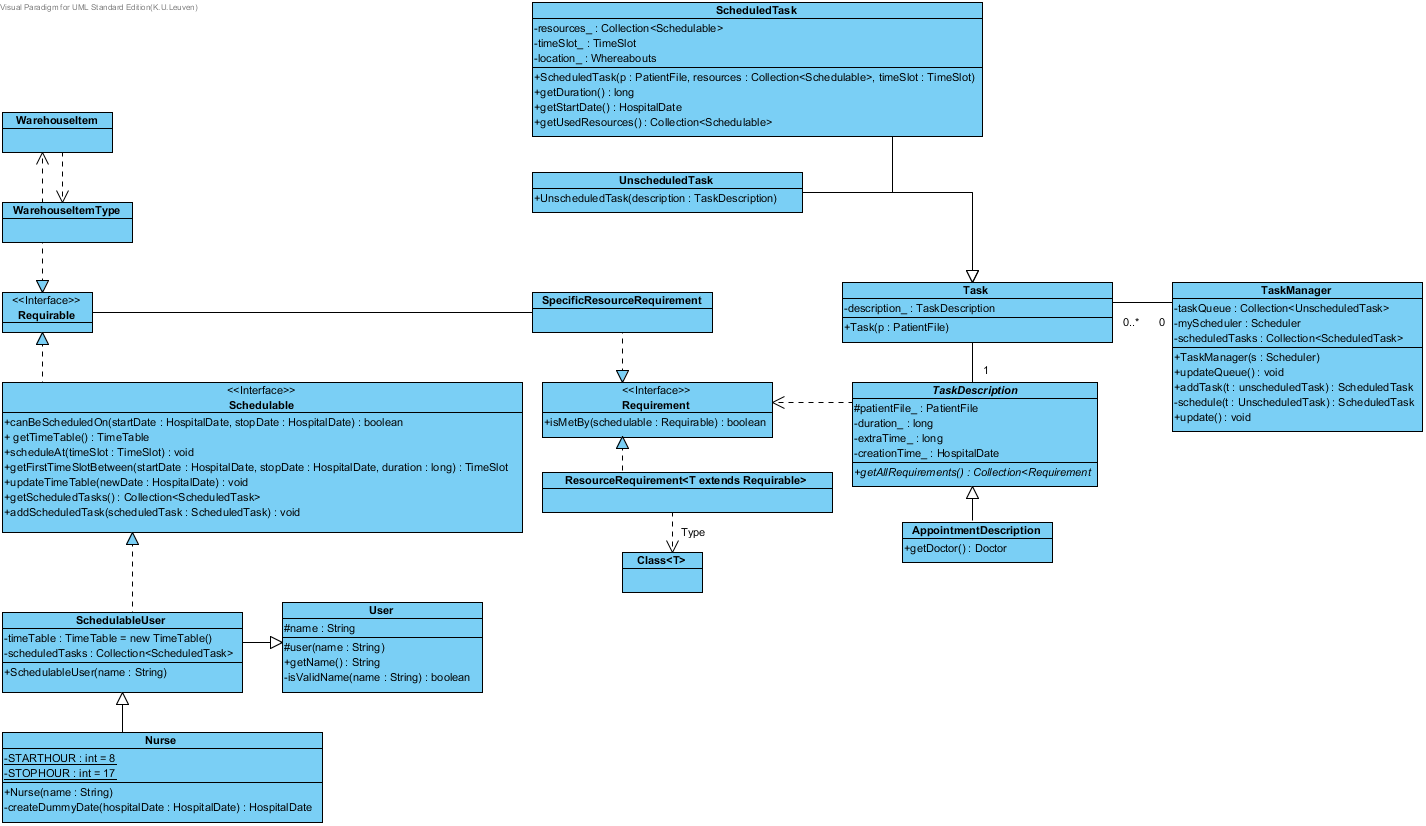
\includegraphics[width=220mm,height=160mm,angle=90]{Task-Description.png}
\caption{Tasks and their descriptions}
\label{taskuml}
\end{figure}

\subsection{The state of a Task}
As described in the beginning of this chapter, tasks undergo "transformations". These transformations are implemented with a state pattern.\\
A task keeps its TaskState. The existing TaskState objects are: QueuedState, ScheduledState, FinishedState. Each state keeps a TaskData object. This object stores information relevant to the current state of the task. For example: a queued task would only keep its description while a scheduled task also keeps all resources involved in the execution of the task, where the task is to take place, etc\dots
\subsection{The description of a Task}
We define tasks by their description. Examples of these descriptions are: blood analysis, surgery, medication, appointment,\dots \\
These descriptions can be created using the controllers and the factories they can provide the user with. Once created, a description gets stored in the task data of a new queued task. A description contains requirements and conditions  specific for that description. These requirements and conditions need to be met in order to schedule the queued task. (see later) You can find a diagram of these states below in figure ~\ref{taskstate} .

\begin{figure}
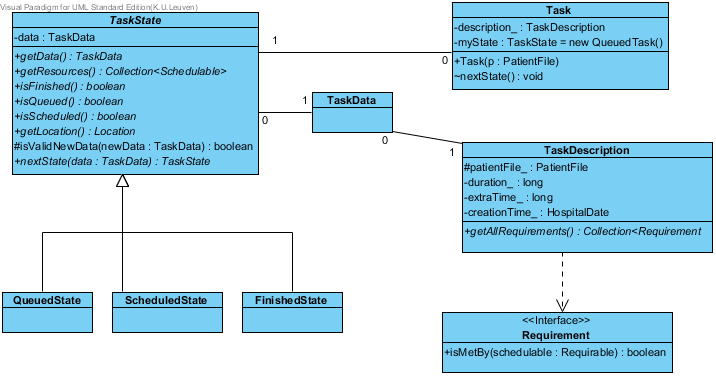
\includegraphics[width=150mm]{TaskState.png}
\caption{Tasks and their states}
\label{taskstate}
\end{figure}

\section{Warehouse}
During this iteration we also made some large refactoring, if not implementing from scratch, from everything related to warehouses. There were a couple of significant problems, like mentioned in the introduction of this report. We managed to successfully find clean solutions for them all.\\
Let's take a look at the class diagram from warehouse first: 

\begin{figure}[h!]
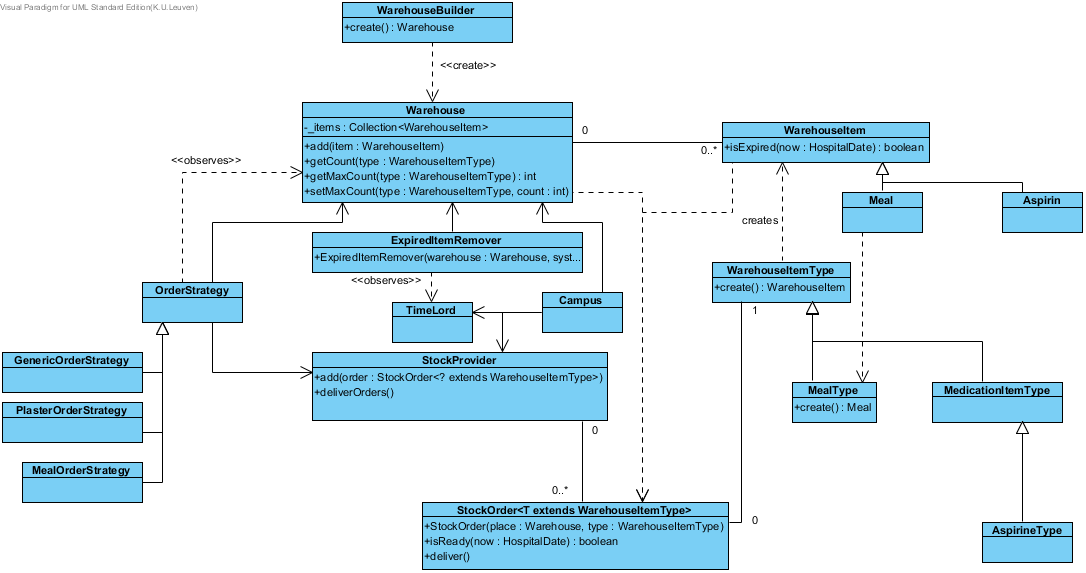
\includegraphics[width=170mm]{Warehouse.png}
\caption{Class diagram from warehouse and its related classes}
\label{warehouse}
\end{figure}

The basic idea is that, using a WarehouseBuilder, we connect an ExpiredItemRemover and as many OrderStrategies to the warehouse as needed.\\ OrderStrategy is a class that, when the item type it's observing is running low, creates new stock orders for the warehouse automatically.\\
As different types require different methods of 
ExpiredItemRemover observes the current system time. Should the time change, the item remover will check if there are items in the warehouse that have expired due to the new system time and will remove them. This removal will, evidently, trigger order strategies to be notified.\\
All newly created stock orders are kept in the stock provider. The stock provider also observes the current system time. When the time changes, the stock provider will attempt to deliver all deliverable stock orders. Stock orders are deliverable if the required time to pass between order creation and the new system time is sufficient.\\
The stock provider is created together with the warehouse and both are stored in the campus. Working with only one stock provider per campus makes it easy to create the exact amount of new stock orders required.\\
The warehouse stores 

\section{Scheduling}
\subsection{Scheduler and task manager}
\subsection{LocationTimeTable and TimeTable}
\subsection{Conditions and requirements}
\subsection{Schedulable and Requirable}
\subsection{Impact of having different locations}
\subsection{The location preference for doctors}
\subsubsection{Preference states}
\subsubsection{getLocationAt()-method}

\section{The updated testing scenario}
We have changed the testing scenario we handed in on the deadline of the refactoring report drastically.
\section{Conclusion}
\end{document}